% Electric Field Lines
% Demonstrates: field lines for point charges, dipoles, and equipotential curves.
% Compile with: pdflatex main.tex

\documentclass[border=10pt]{standalone}
\usepackage{tikz}
\usetikzlibrary{arrows.meta, decorations.markings, calc}

\begin{document}
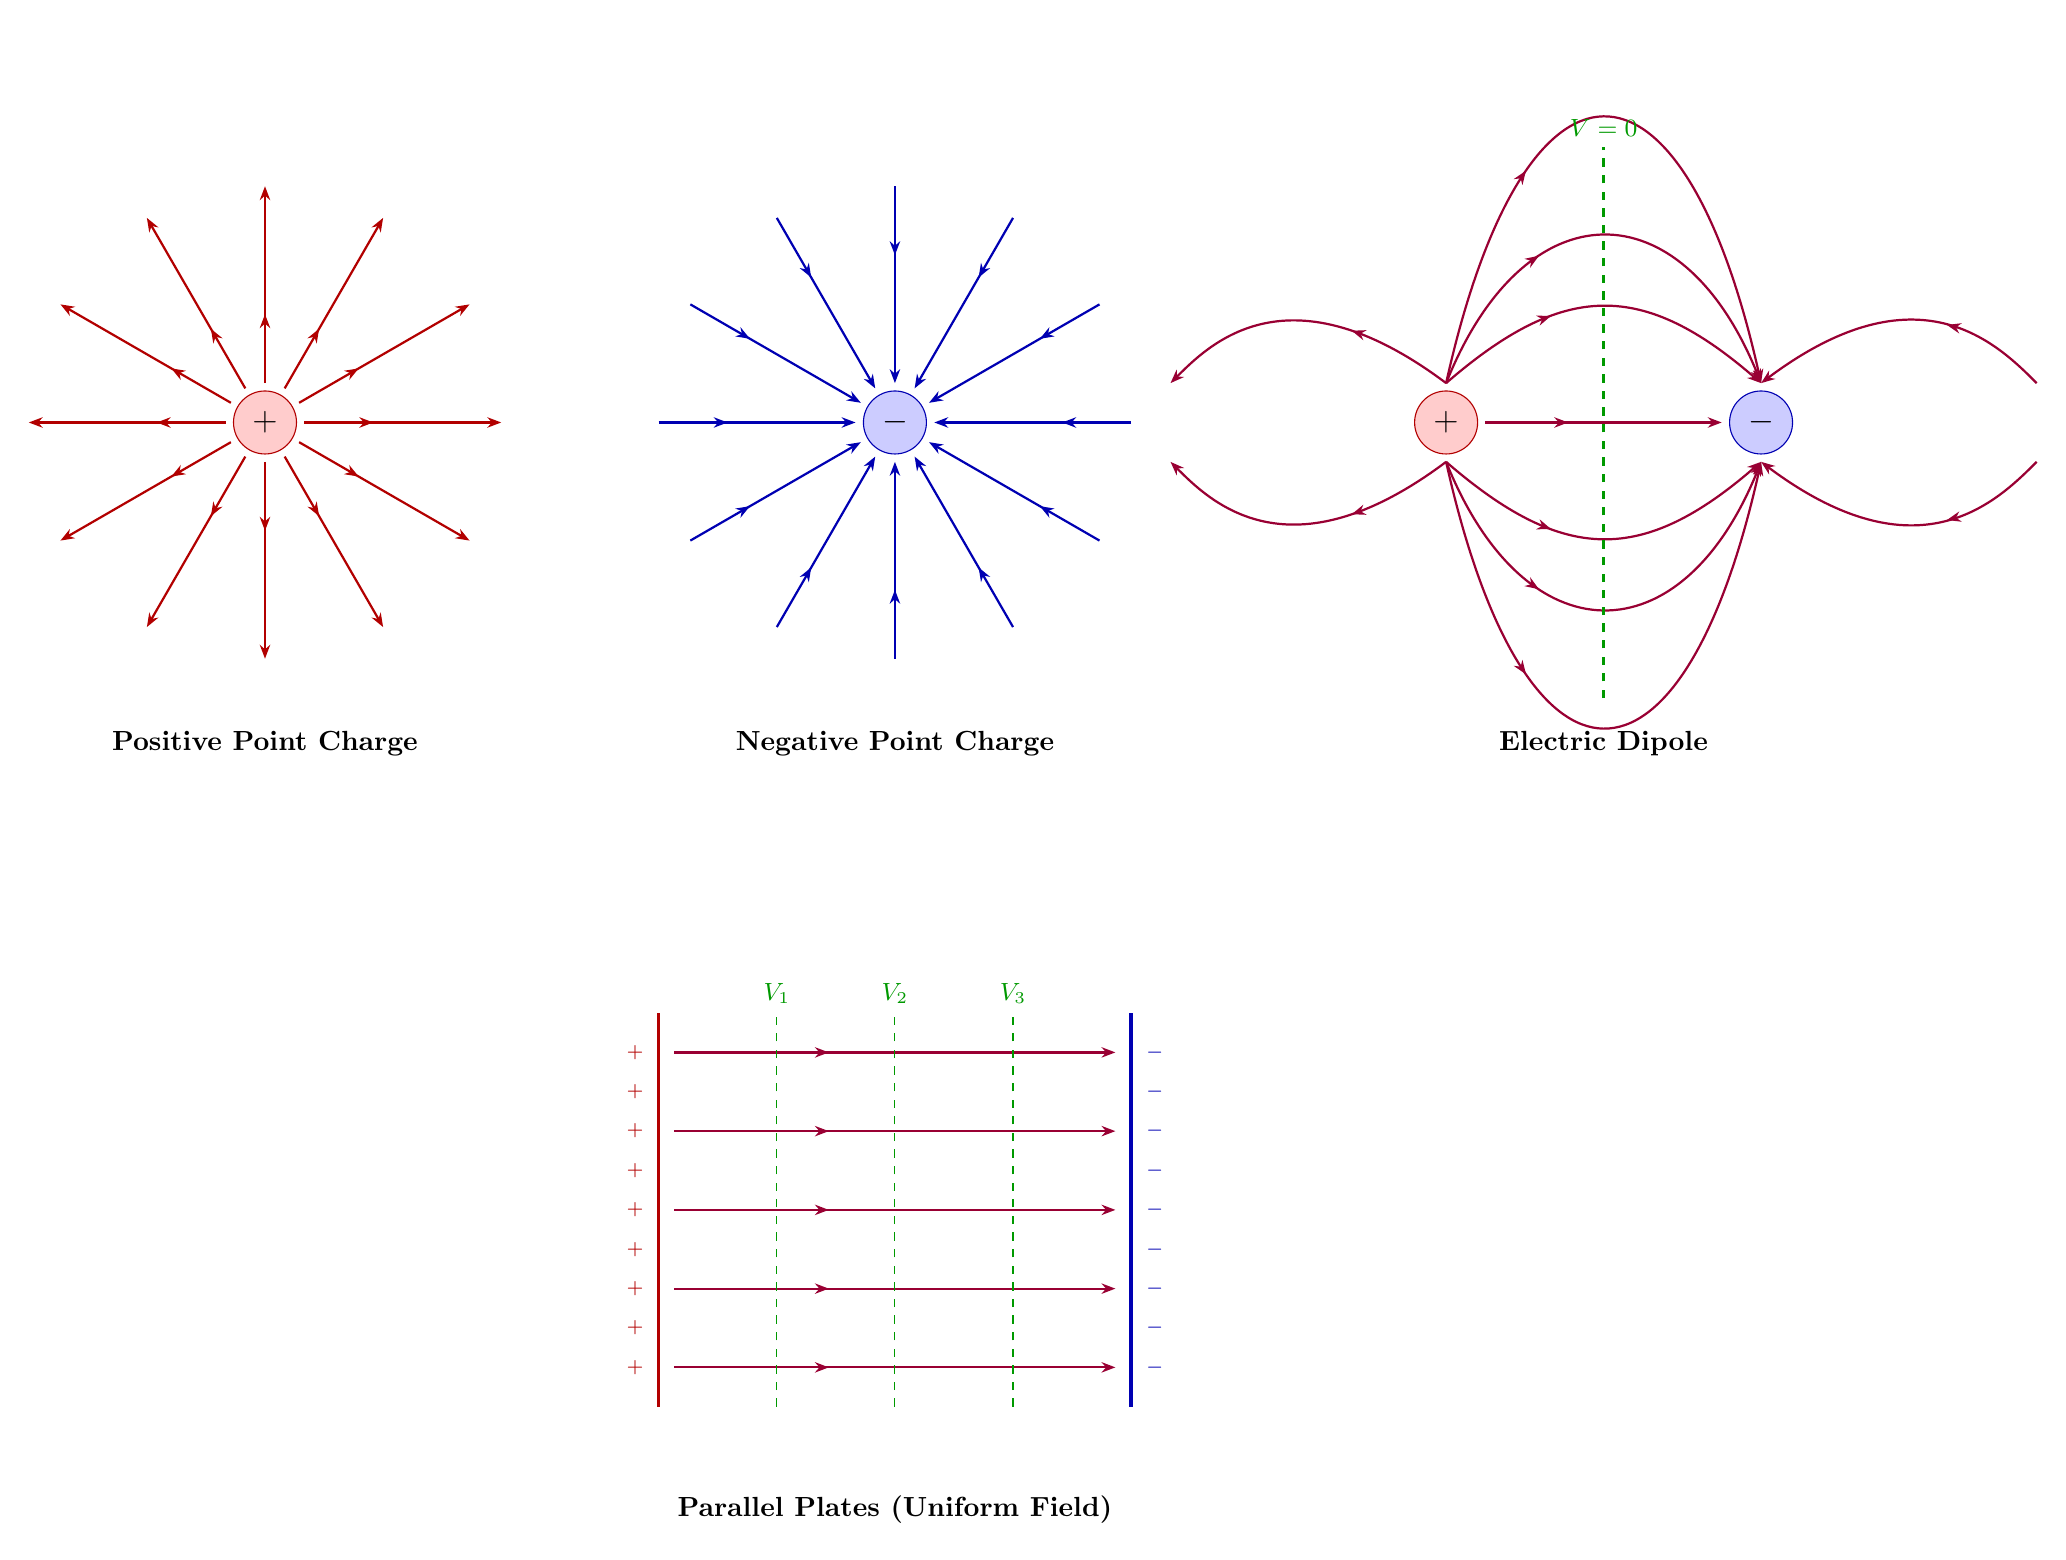
\begin{tikzpicture}[
    field/.style={
        thick, -{Stealth[length=5pt]},
        postaction={decorate, decoration={
            markings,
            mark=at position 0.35 with {\arrow{Stealth[length=5pt]}},
        }},
    },
    charge+/.style={circle, draw=red!70!black, fill=red!20, minimum size=8mm,
        font=\bfseries\large, inner sep=0pt},
    charge-/.style={circle, draw=blue!70!black, fill=blue!20, minimum size=8mm,
        font=\bfseries\large, inner sep=0pt},
]

% =============================================================================
% Scene 1: Single positive charge
% =============================================================================
\begin{scope}[shift={(0,0)}]
    \node[charge+] (q) at (0,0) {$+$};

    % Radial field lines outward
    \foreach \a in {0, 30, 60, ..., 330} {
        \draw[field, red!70!black] (0,0) ++(\a:0.5) -- ++(\a:2.5);
    }

    \node[font=\bfseries, anchor=north] at (0, -3.8) {Positive Point Charge};
\end{scope}

% =============================================================================
% Scene 2: Single negative charge
% =============================================================================
\begin{scope}[shift={(8,0)}]
    \node[charge-] (q) at (0,0) {$-$};

    % Radial field lines inward
    \foreach \a in {0, 30, 60, ..., 330} {
        \draw[field, blue!70!black] (\a:3) -- (\a:0.5);
    }

    \node[font=\bfseries, anchor=north] at (0, -3.8) {Negative Point Charge};
\end{scope}

% =============================================================================
% Scene 3: Electric dipole
% =============================================================================
\begin{scope}[shift={(17,0)}]

    \node[charge+] (p) at (-2, 0) {$+$};
    \node[charge-] (n) at (2, 0) {$-$};

    % Field lines from + to - (curved paths)
    % Top lines
    \draw[field, purple!80!black]
        (-2, 0.5) .. controls (-1, 3) and (1, 3) .. (2, 0.5);
    \draw[field, purple!80!black]
        (-2, 0.5) .. controls (-0.5, 1.8) and (0.5, 1.8) .. (2, 0.5);
    \draw[field, purple!80!black]
        (-2, 0.5) .. controls (-1, 5) and (1, 5) .. (2, 0.5);

    % Bottom lines (mirror)
    \draw[field, purple!80!black]
        (-2, -0.5) .. controls (-1, -3) and (1, -3) .. (2, -0.5);
    \draw[field, purple!80!black]
        (-2, -0.5) .. controls (-0.5, -1.8) and (0.5, -1.8) .. (2, -0.5);
    \draw[field, purple!80!black]
        (-2, -0.5) .. controls (-1, -5) and (1, -5) .. (2, -0.5);

    % Straight line through center
    \draw[field, purple!80!black] (-1.5, 0) -- (1.5, 0);

    % External lines going to infinity
    \draw[field, purple!80!black]
        (-2, 0.5) .. controls (-4, 2) and (-5, 1) .. (-5.5, 0.5);
    \draw[field, purple!80!black]
        (-2, -0.5) .. controls (-4, -2) and (-5, -1) .. (-5.5, -0.5);
    \draw[field, purple!80!black]
        (5.5, 0.5) .. controls (5, 1) and (4, 2) .. (2, 0.5);
    \draw[field, purple!80!black]
        (5.5, -0.5) .. controls (5, -1) and (4, -2) .. (2, -0.5);

    % Equipotential lines (dashed, perpendicular to field)
    \draw[dashed, green!60!black, thick] (0, -3.5) -- (0, 3.5)
        node[above, font=\small] {$V = 0$};

    \node[font=\bfseries, anchor=north] at (0, -3.8) {Electric Dipole};
\end{scope}

% =============================================================================
% Scene 4: Parallel plates (uniform field)
% =============================================================================
\begin{scope}[shift={(8, -10)}]

    % Positive plate
    \draw[very thick, red!70!black] (-3, -2.5) -- (-3, 2.5);
    \foreach \y in {-2, -1.5, ..., 2} {
        \node[font=\scriptsize, red!70!black] at (-3.3, \y) {$+$};
    }

    % Negative plate
    \draw[very thick, blue!70!black] (3, -2.5) -- (3, 2.5);
    \foreach \y in {-2, -1.5, ..., 2} {
        \node[font=\scriptsize, blue!70!black] at (3.3, \y) {$-$};
    }

    % Uniform field lines
    \foreach \y in {-2, -1, 0, 1, 2} {
        \draw[field, purple!80!black] (-2.8, \y) -- (2.8, \y);
    }

    % Equipotential lines
    \foreach \x in {-1.5, 0, 1.5} {
        \draw[dashed, green!60!black] (\x, -2.5) -- (\x, 2.5);
    }

    \node[font=\small, green!60!black, above] at (-1.5, 2.5) {$V_1$};
    \node[font=\small, green!60!black, above] at (0, 2.5) {$V_2$};
    \node[font=\small, green!60!black, above] at (1.5, 2.5) {$V_3$};

    \node[font=\bfseries, anchor=north] at (0, -3.5) {Parallel Plates (Uniform Field)};
\end{scope}

\end{tikzpicture}
\end{document}
